\subsection{Sensors characterization}
\label{subsec:sensors_characterization}

In this subsection, we will focus on the characterization of the sensors used internally by the control unit to measure or estimate the system state.



\subsubsection{Voltage to position mapping}
\label{subsubsec:voltage_to_position}

At first, we need to create the mapping between the voltage output of the infrared sensor and the position of the ball.
To do so, we simply sample the output voltage of the infrared sensor and the position of the ball using the data acquisition system included in the \texttt{Inteco} control unit and a caliper.

The obtained data is shown in Figure \ref{fig:voltage_to_position}.

\begin{figure}[H]
    \centering
    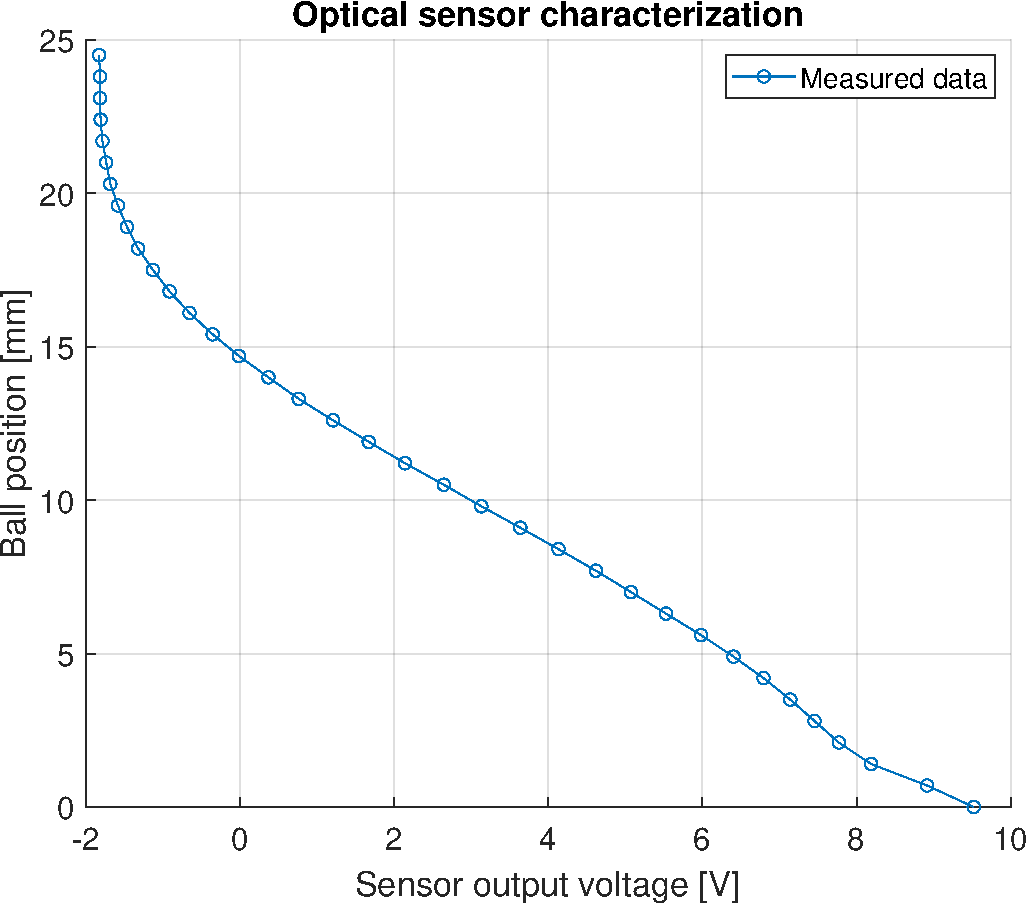
\includegraphics[width=0.6\textwidth]{img/MATLAB/identification/sensor_position.pdf}
    \caption{Position of the ball as a function of the output voltage of the infrared optical sensor.}
    \label{fig:voltage_to_position}
\end{figure}

One can clearly see the non-linear relationship between the ball's position and the output voltage of the infrared sensor.

Moreover, it's important to underline the hardware limitations of the sensor that allows a maximum measurement distance of $\approx 20 [mm]$ from the upper coil before reaching its saturation limit.



\subsubsection{Sensors noise analysis}
\label{subsubsec:sensors_noise}

A comprehensive analysis of the sensors' noise is crucial to correctly estimate both the position of the ball and the coils' current.
The experimental setup consists of keeping the ball at a fixed position and recording the sensors' output for a certain amount of time imposing a zero control signal.
The analysis then assumes the sensors' noise to be a zero-mean Gaussian white noise process.

With this optics, we can estimate the standard deviation for each sensor and use it to design the filters and estimators in the following sections (see Section \ref{sec:filters_estimators_design}).

\begin{figure}[H]
    \centering
    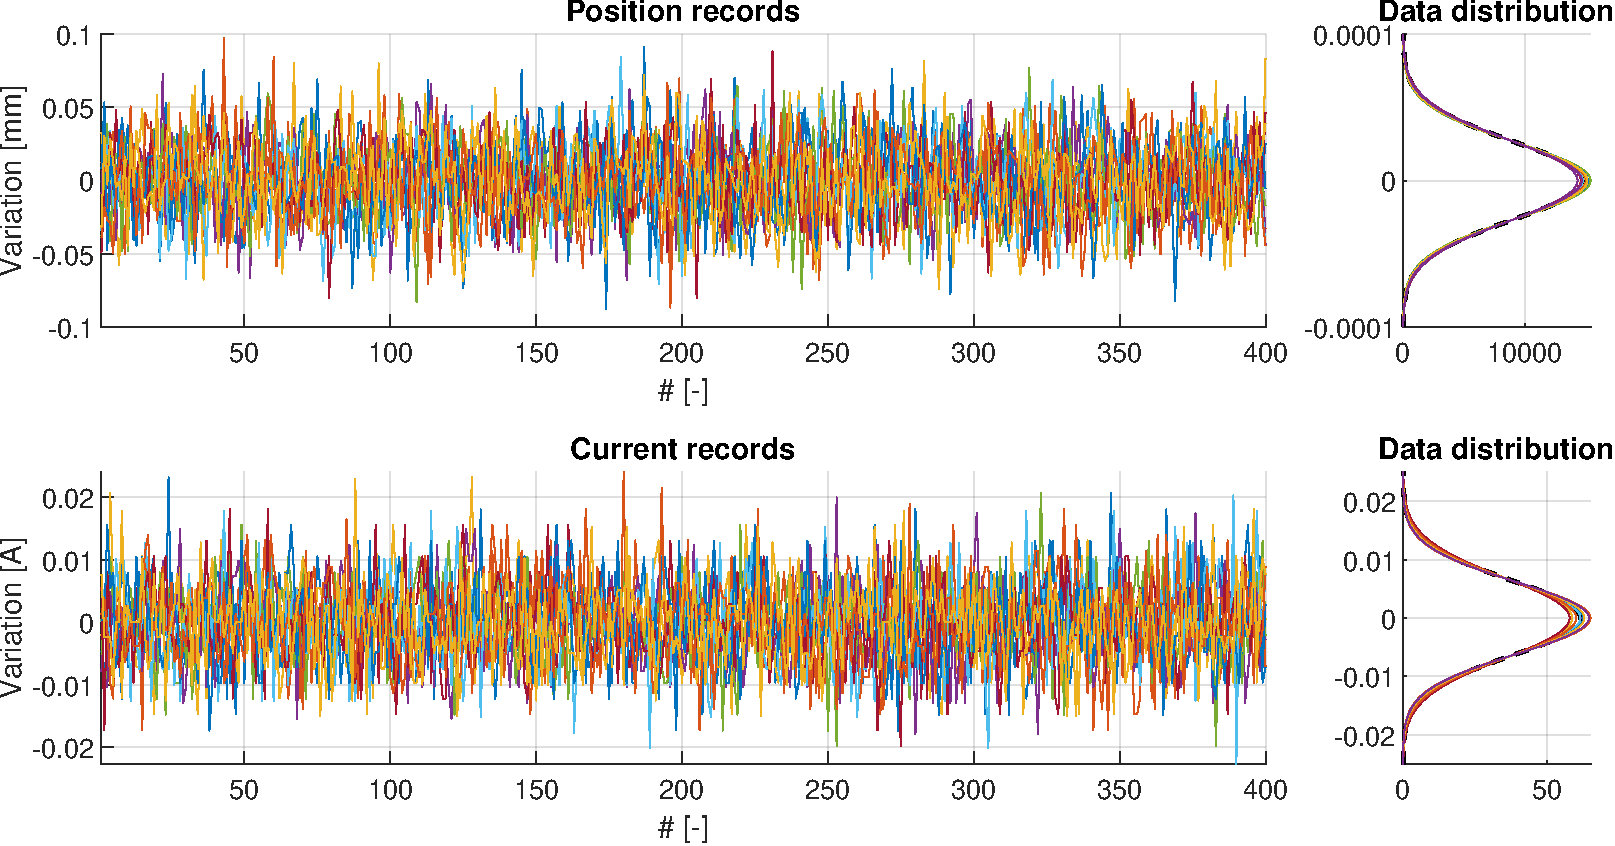
\includegraphics[width=1\textwidth]{img/MATLAB/identification/sensor_noises.pdf}
    \caption{Sensors' noise analysis.}
    \label{fig:sensors_noise}
\end{figure}

In Figure \ref{fig:sensors_noise}, the analysis of the sensors' noise is shown.

The left plots show the time history of the sensor output variations, while the right plots show the Gaussian distribution of the sensors' noise with the mean distribution marked with a dashed black line.
The upper plots refer to the infrared sensor, while the lower plots refer to the current sensor.

The standard deviation and covariance of the sensors' noise is reported in Table \ref{tab:sensors_noise}.

\begin{table}[H]
    \centering

    \begin{tabular}{|c|c|c|}
        \hline
        \textbf{Sensor} & \textbf{Standard deviation}        & \textbf{Covariance}                  \\
        \hline
        Infrared        & $1.402804 \cdot 10^{-3} \quad [m]$ & $7.166031 \cdot 10^{-6} \quad [m^2]$ \\
        Current         & $6.327979 \cdot 10^{-3} \quad [A]$ & $4.005490 \cdot 10^{-5} \quad [A^2]$ \\
        \hline
    \end{tabular}

    \caption{Standard deviation and covariance of the sensors' noise.}
    \label{tab:sensors_noise}

\end{table}
